% !TeX program = pdflatex
\documentclass[12pt,a4paper]{article}

\usepackage[margin=25mm]{geometry}
\usepackage[T1]{fontenc}
\usepackage[utf8]{inputenc}
\usepackage{lmodern}
\usepackage{graphicx}
\usepackage{amsmath,amssymb}
\usepackage{booktabs}
\usepackage{tabularx}
\usepackage{array}
\usepackage{float}
\usepackage{subcaption}
\usepackage{hyperref}
\usepackage{fancyhdr}
\usepackage{titlesec}
\usepackage{xcolor}
\usepackage{siunitx}

\graphicspath{{./}{figures/}}
\hypersetup{colorlinks=true,linkcolor=black,urlcolor=blue,citecolor=black}
\pagestyle{fancy}
\fancyhf{}
\lhead{Biomechanics}
\rhead{EMG Practical}
\cfoot{\thepage}
\setlength{\headheight}{15pt}
\titleformat{\section}{\Large\bfseries}{\thesection}{0.7em}{}
\titleformat{\subsection}{\large\bfseries}{\thesubsection}{0.7em}{}
\newcommand{\csvfile}[1]{\texttt{\detokenize{#1}}}
\newcommand{\uV}{\ensuremath{\,\mu\mathrm{V}}}
\sisetup{group-separator={,},group-minimum-digits=4}

\begin{document}

\hypersetup{pageanchor=false}
\begin{titlepage}
  \centering
  \vspace*{7mm}
  \IfFileExists{campus_logo.png}{
\includegraphics[width=4.2cm]{campus_logo.png}\par\vspace{7mm}}{\vspace{12mm}}
  {\large University of Moratuwa\par}
  \vspace{18mm}
  {\large B.Sc. Engineering (Hons)\par}
  \vspace{5mm}
  {\Large\bfseries Department of Mechanical Engineering\par}
  \vspace{15mm}
  {\Huge\bfseries EMG Practical Report\par}
  \vspace{5mm}
  {\LARGE Surface EMG Response to 1 kg and 2 kg Loads\par}
  \vspace{3mm}
  {\large Raw Signal Analysis, RMS Feature Extraction, and MVC Referencing\par}
  \vfill
  \renewcommand{\arraystretch}{1.35}
  \begin{tabular}{rl}
    \textbf{Module Code:} & BM3500 \\
    \textbf{Module Title:} & Biomedical Engineering Applications \\
    \textbf{Laboratory:} & Bionics Laboratory \\
    \textbf{Assignment:} & Electromyography signal acquisition and interpretation \\
    \textbf{Student Name \& Index:} & Nuwanaka W.A.S. (230449N) \\
    \textbf{Facilitators:} & Ms. E.M.A.I. Ekanayake, Mrs. N.B.N. Nuwarapaksha \\
    \textbf{Date:} & \today \\
  \end{tabular}
  \vfill
  {\large \today\par}
\end{titlepage}
\hypersetup{pageanchor=true}
\pagenumbering{roman}
\tableofcontents
\newpage
\pagenumbering{arabic}

\section{Introduction}
Electromyography (EMG) measures the electrical activity associated with skeletal-muscle
activation. Surface EMG is a non-invasive measurement used in biomechanics to examine
activation timing and relative muscle effort. Since raw EMG oscillates rapidly around a
baseline and is affected by noise and electrode placement, an amplitude envelope such as
root mean square (RMS) is useful for summarising activity over short time windows.

The purpose of this practical was to inspect surface-EMG recordings made under two
external loads, 1 kg and 2 kg, and to compare their signal amplitudes using a consistent
RMS window. A supplied maximum voluntary contraction (MVC) sliding-RMS recording was
also used as a reference for expressing trial activity relative to the recorded MVC peak.
Only the 1 kg and 2 kg load conditions are discussed in this report; the files are treated
as repeated recordings within those two conditions, not as four different load levels.

\section{Methods}
\subsection{Apparatus and acquisition}
The experiment used a surface EMG sensor connected to an acquisition system and a
computer-based data-capture interface. The exported metadata identifies EMG sensor 4,
Channel 4, with a sampling frequency of \(4000\,\mathrm{Hz}\), voltage units, and a time
base in seconds. The four supplied raw recordings and one MVC sliding-RMS recording are
summarised in Table~\ref{tab:data-files}.

\begin{table}[H]
\centering
\caption{EMG files used and the two load conditions represented in this report.}
\label{tab:data-files}
\small
\begin{tabularx}{\textwidth}{>{\raggedright\arraybackslash}p{0.42\textwidth} >{\centering\arraybackslash}p{0.12\textwidth} >{\centering\arraybackslash}p{0.15\textwidth} >{\centering\arraybackslash}X}
\toprule
\textbf{File} & \textbf{Load} & \textbf{Samples} & \textbf{Duration (s)} \\
\midrule
\csvfile{emg_raw_trial_16.csv} & 1 kg & 82,000 & 20.50 \\
\csvfile{emg_raw_trial_19.csv} & 1 kg & 82,000 & 20.50 \\
\csvfile{emg_raw_trial_27.csv} & 2 kg & 8,000 & 2.00 \\
\csvfile{emg_raw_trial_38.csv} & 2 kg & 82,000 & 20.50 \\
\csvfile{emg_mvc_sliding_rms.csv} & MVC reference & 110,000 & 27.50 \\
\bottomrule
\end{tabularx}
\end{table}

\noindent\textbf{Load-label note.} The CSV metadata contains sensor, sampling-rate, and sample-count information, but does not contain a field identifying the applied mass. For the current plots, the trial files are grouped in acquisition-number order as trial 16 and trial 19 for 1 kg, and trial 27 and trial 38 for 2 kg. This assignment must be checked against the laboratory notes. If the trial-to-load pairing in the lab record differs, edit the \texttt{LOAD\_GROUPS} mapping near the top of \csvfile{emg\_generate\_figures.py} and regenerate the graphs before submission.

\subsection{Electrode placement and subject instruction}
The skin over the target muscle was prepared before electrode attachment to reduce
contact impedance. The active electrodes were placed over the target muscle belly and
aligned with the muscle-fibre direction, while the reference electrode was placed over
an electrically quiet bony area. The subject was asked to perform the movement with each
load while minimising unnecessary body movement. Rest periods were allowed between
trials, and the activity was stopped if discomfort occurred.

\subsection{RMS feature extraction}
For the raw recordings, the mean of each trace was subtracted before calculating a
centred 100 ms moving RMS envelope. At a sampling frequency of \(4000\,\mathrm{Hz}\), a
100 ms window contains \(N=400\) samples. The RMS at sample \(n\) is
\begin{equation}
  \mathrm{RMS}[n]
  = \sqrt{\frac{1}{N}\sum_{k=0}^{N-1}x_c^2[n-k]},
  \label{eq:rms}
\end{equation}
where \(x_c\) is the raw signal after removal of its mean. This procedure gives a positive
amplitude envelope while retaining the broad timing of muscle activation. The edges of
short recordings contain fewer samples in their moving windows.

\subsection{MVC referencing}
The supplied MVC file is already exported as a sliding-RMS signal. Trial RMS amplitudes
were expressed relative to the maximum value of that provided MVC trace:
\begin{equation}
  \text{MVC-referenced activity}[n]
  = \frac{\mathrm{RMS}_{\text{trial}}[n]}
  {\max(\mathrm{RMS}_{\text{MVC, supplied}})}\times 100\%.
  \label{eq:mvc}
\end{equation}
The MVC-referenced values are an approximate comparison because the CSV export does not
fully document the internal window settings used to generate the supplied MVC signal.
They should not be interpreted as a clinical measurement or as a force estimate.

\section{Results}
\subsection{Raw EMG signals}
Figure~\ref{fig:raw-emg} shows the raw voltage signals for both load conditions. The
plots display the first five seconds where available so the waveforms can be viewed on a
comparable time scale. Trial 27 contains only 2.00 seconds of data, whereas the other
raw recordings contain 20.50 seconds. The shorter recording therefore provides less
temporal evidence and should be interpreted cautiously.

\begin{figure}[H]
  \centering
  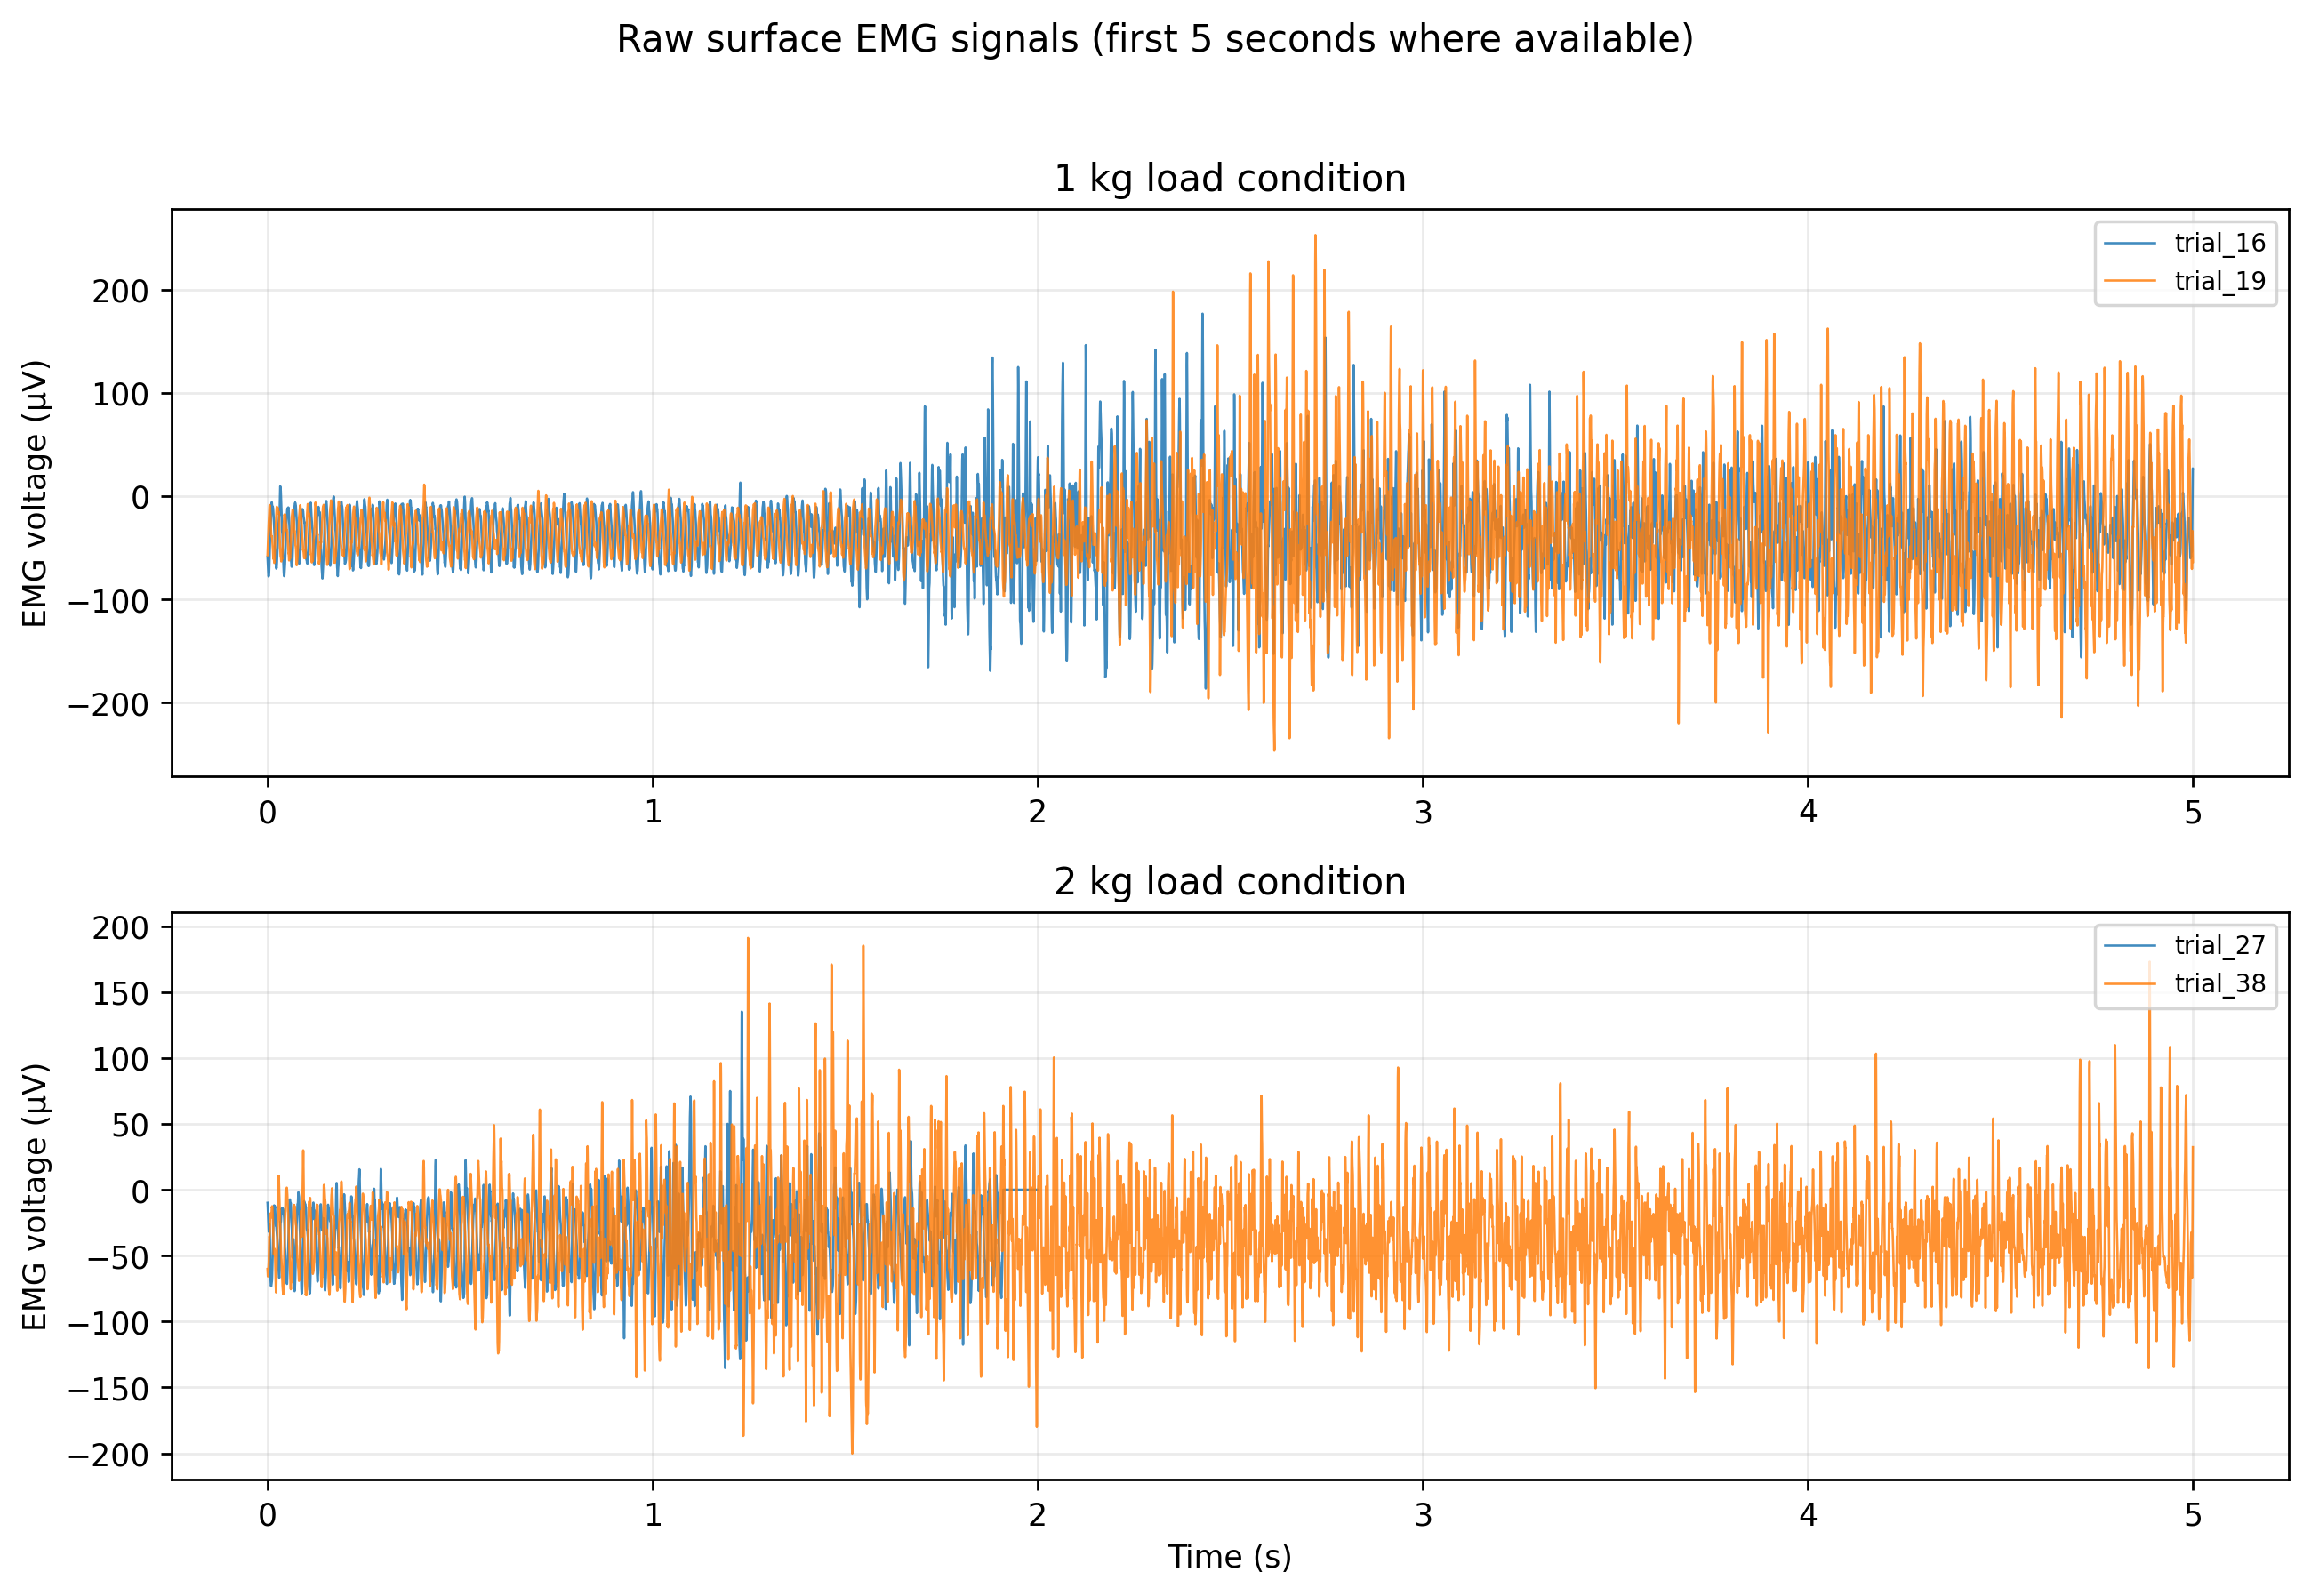
\includegraphics[width=0.96\textwidth]{emg_raw_loads.png}
  \caption{Raw EMG voltage traces grouped into the 1 kg and 2 kg load conditions. Traces are shown in microvolts; the plotted interval is limited to the first five seconds where available.}
  \label{fig:raw-emg}
\end{figure}

\subsection{RMS envelopes}
Figure~\ref{fig:rms-emg} shows the 100 ms moving RMS envelopes. RMS smoothing reduces
rapid sign changes in the raw EMG and makes changes in signal amplitude easier to inspect.
The figure retains the individual recordings instead of averaging them into a single
curve, allowing trial-to-trial differences to remain visible.

\begin{figure}[H]
  \centering
  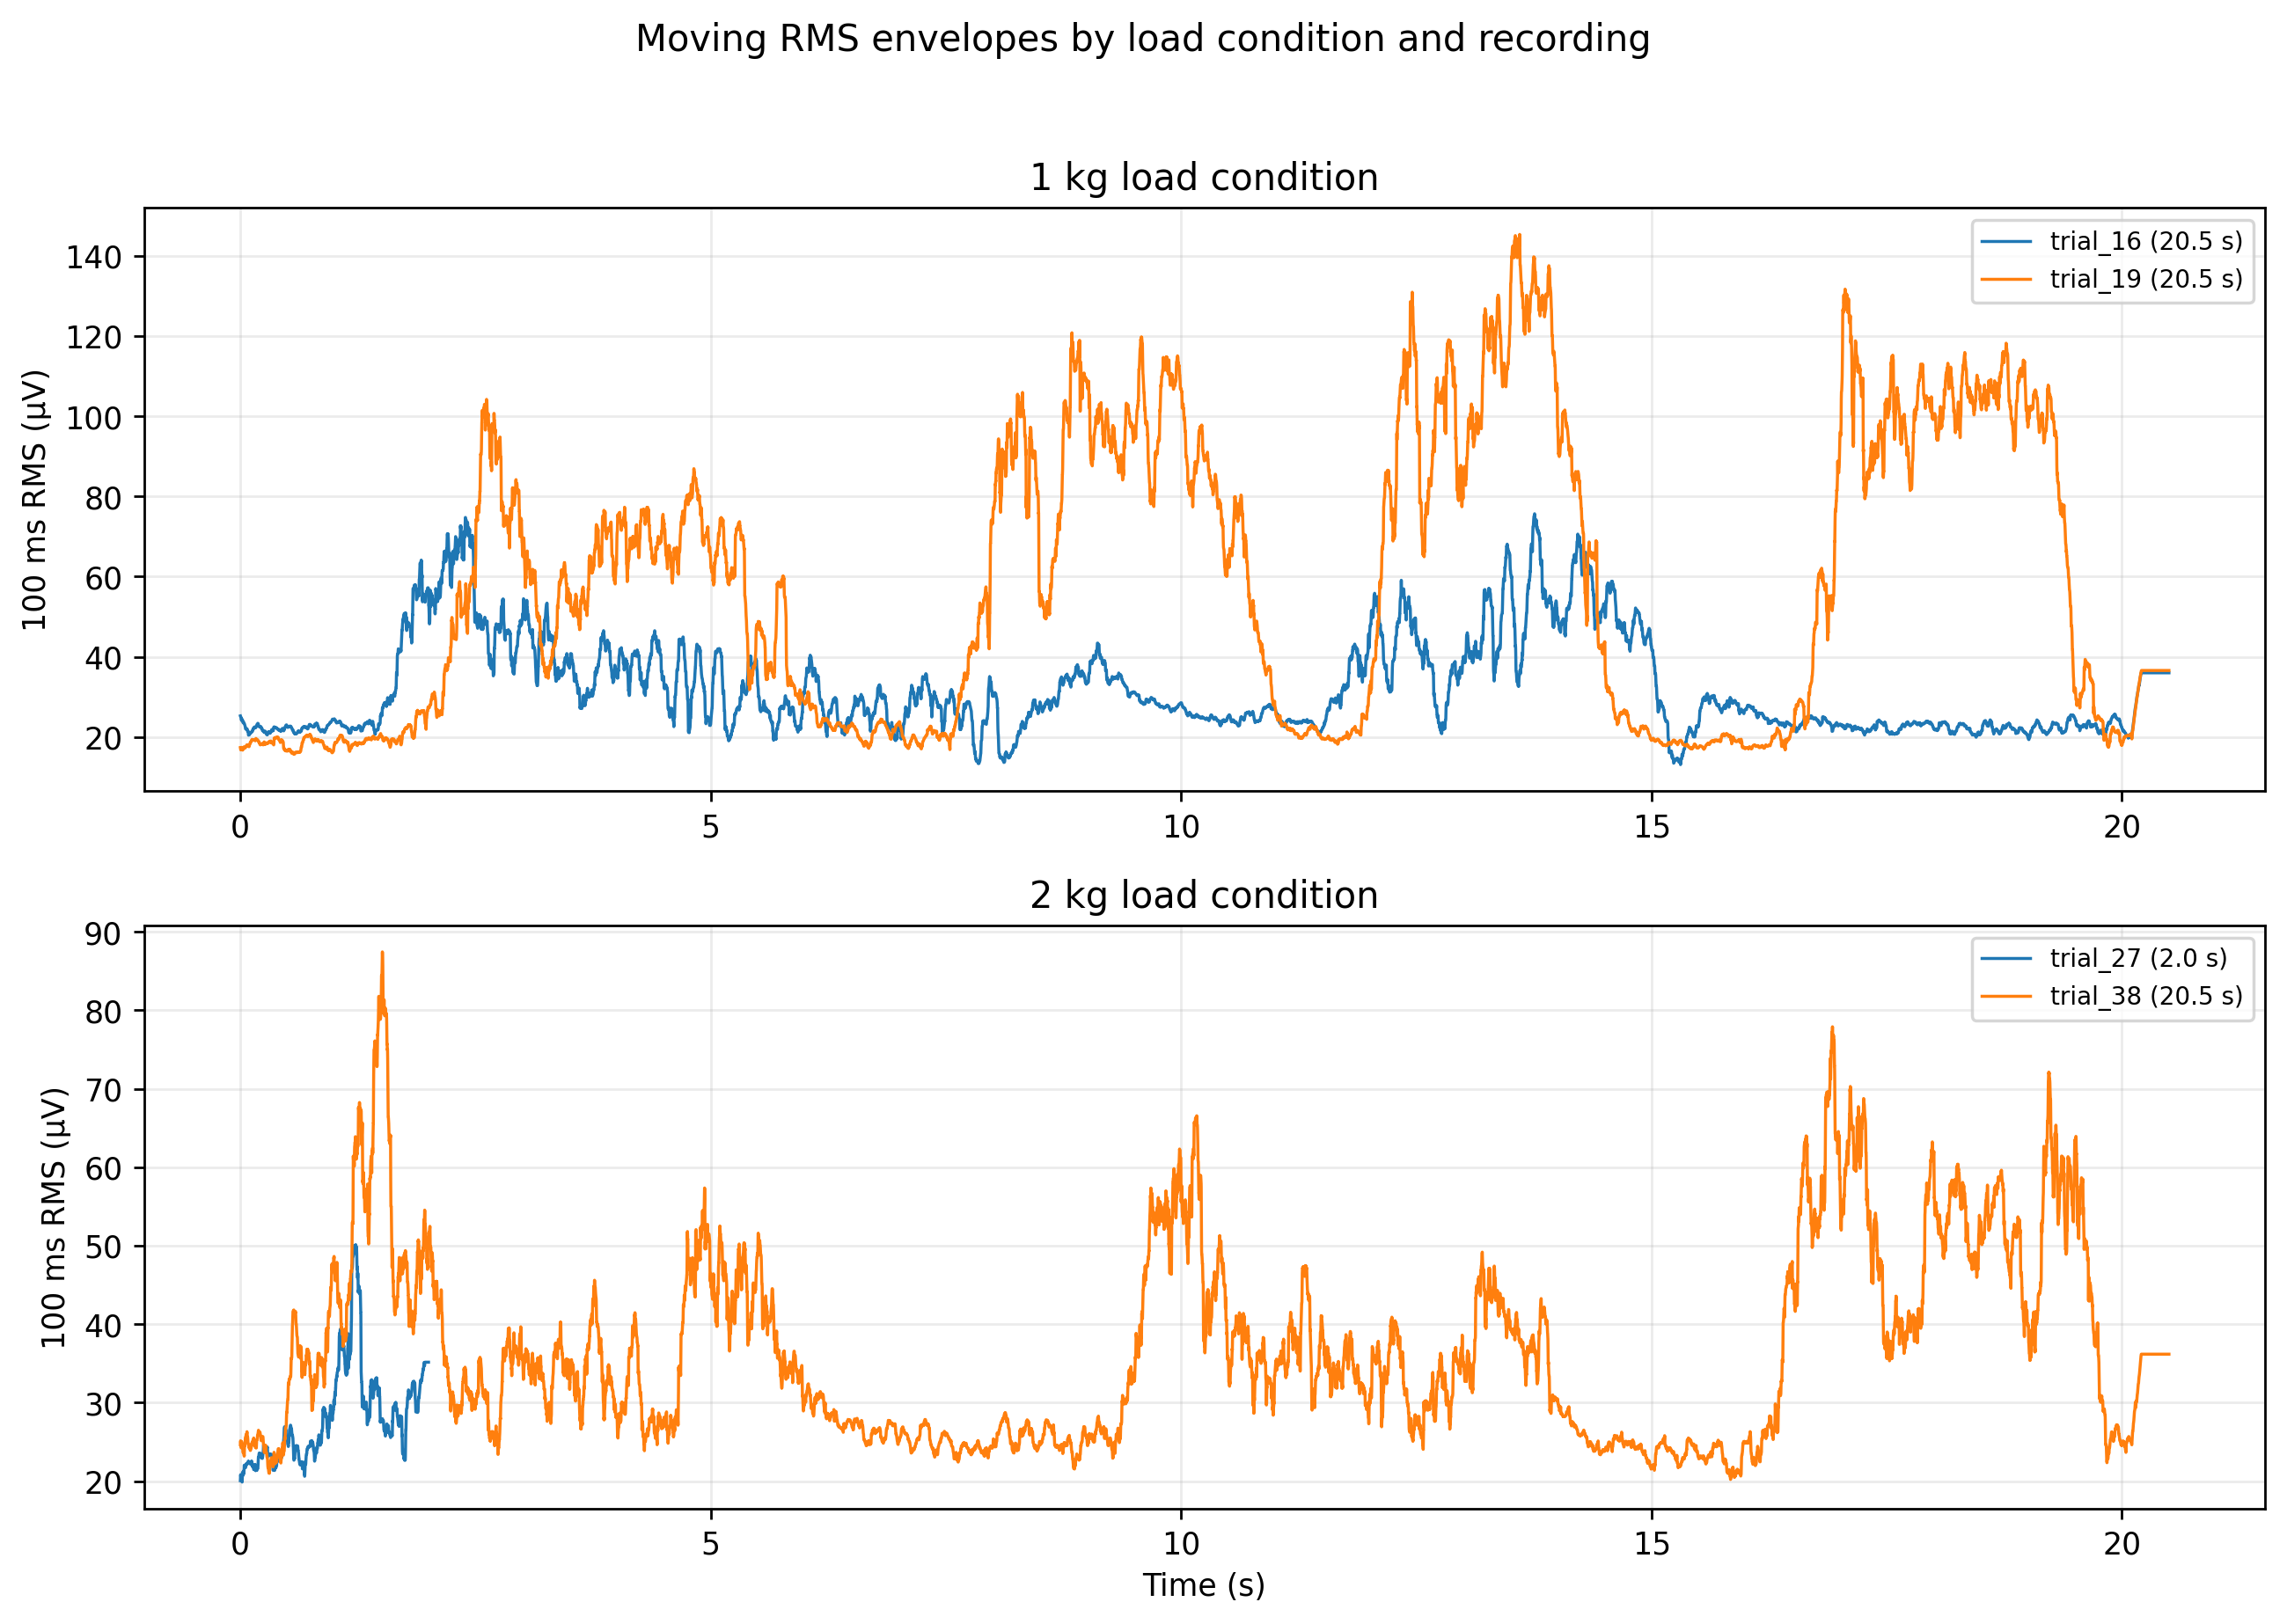
\includegraphics[width=0.96\textwidth]{emg_rms_loads.png}
  \caption{100 ms moving RMS envelopes for the individual recordings grouped under the 1 kg and 2 kg conditions.}
  \label{fig:rms-emg}
\end{figure}

\subsection{MVC reference and normalised activity}
The provided MVC sliding-RMS trace is shown in Figure~\ref{fig:mvc-reference}. Its
maximum exported value is approximately \(402.65\uV\), which is used as the denominator
for the MVC-referenced traces in Figure~\ref{fig:mvc-normalised}. Because the reference
signal was preprocessed by the acquisition software, the normalised curves are best
regarded as relative amplitude indicators rather than perfectly standardised \%MVC
measurements.

\begin{figure}[H]
  \centering
  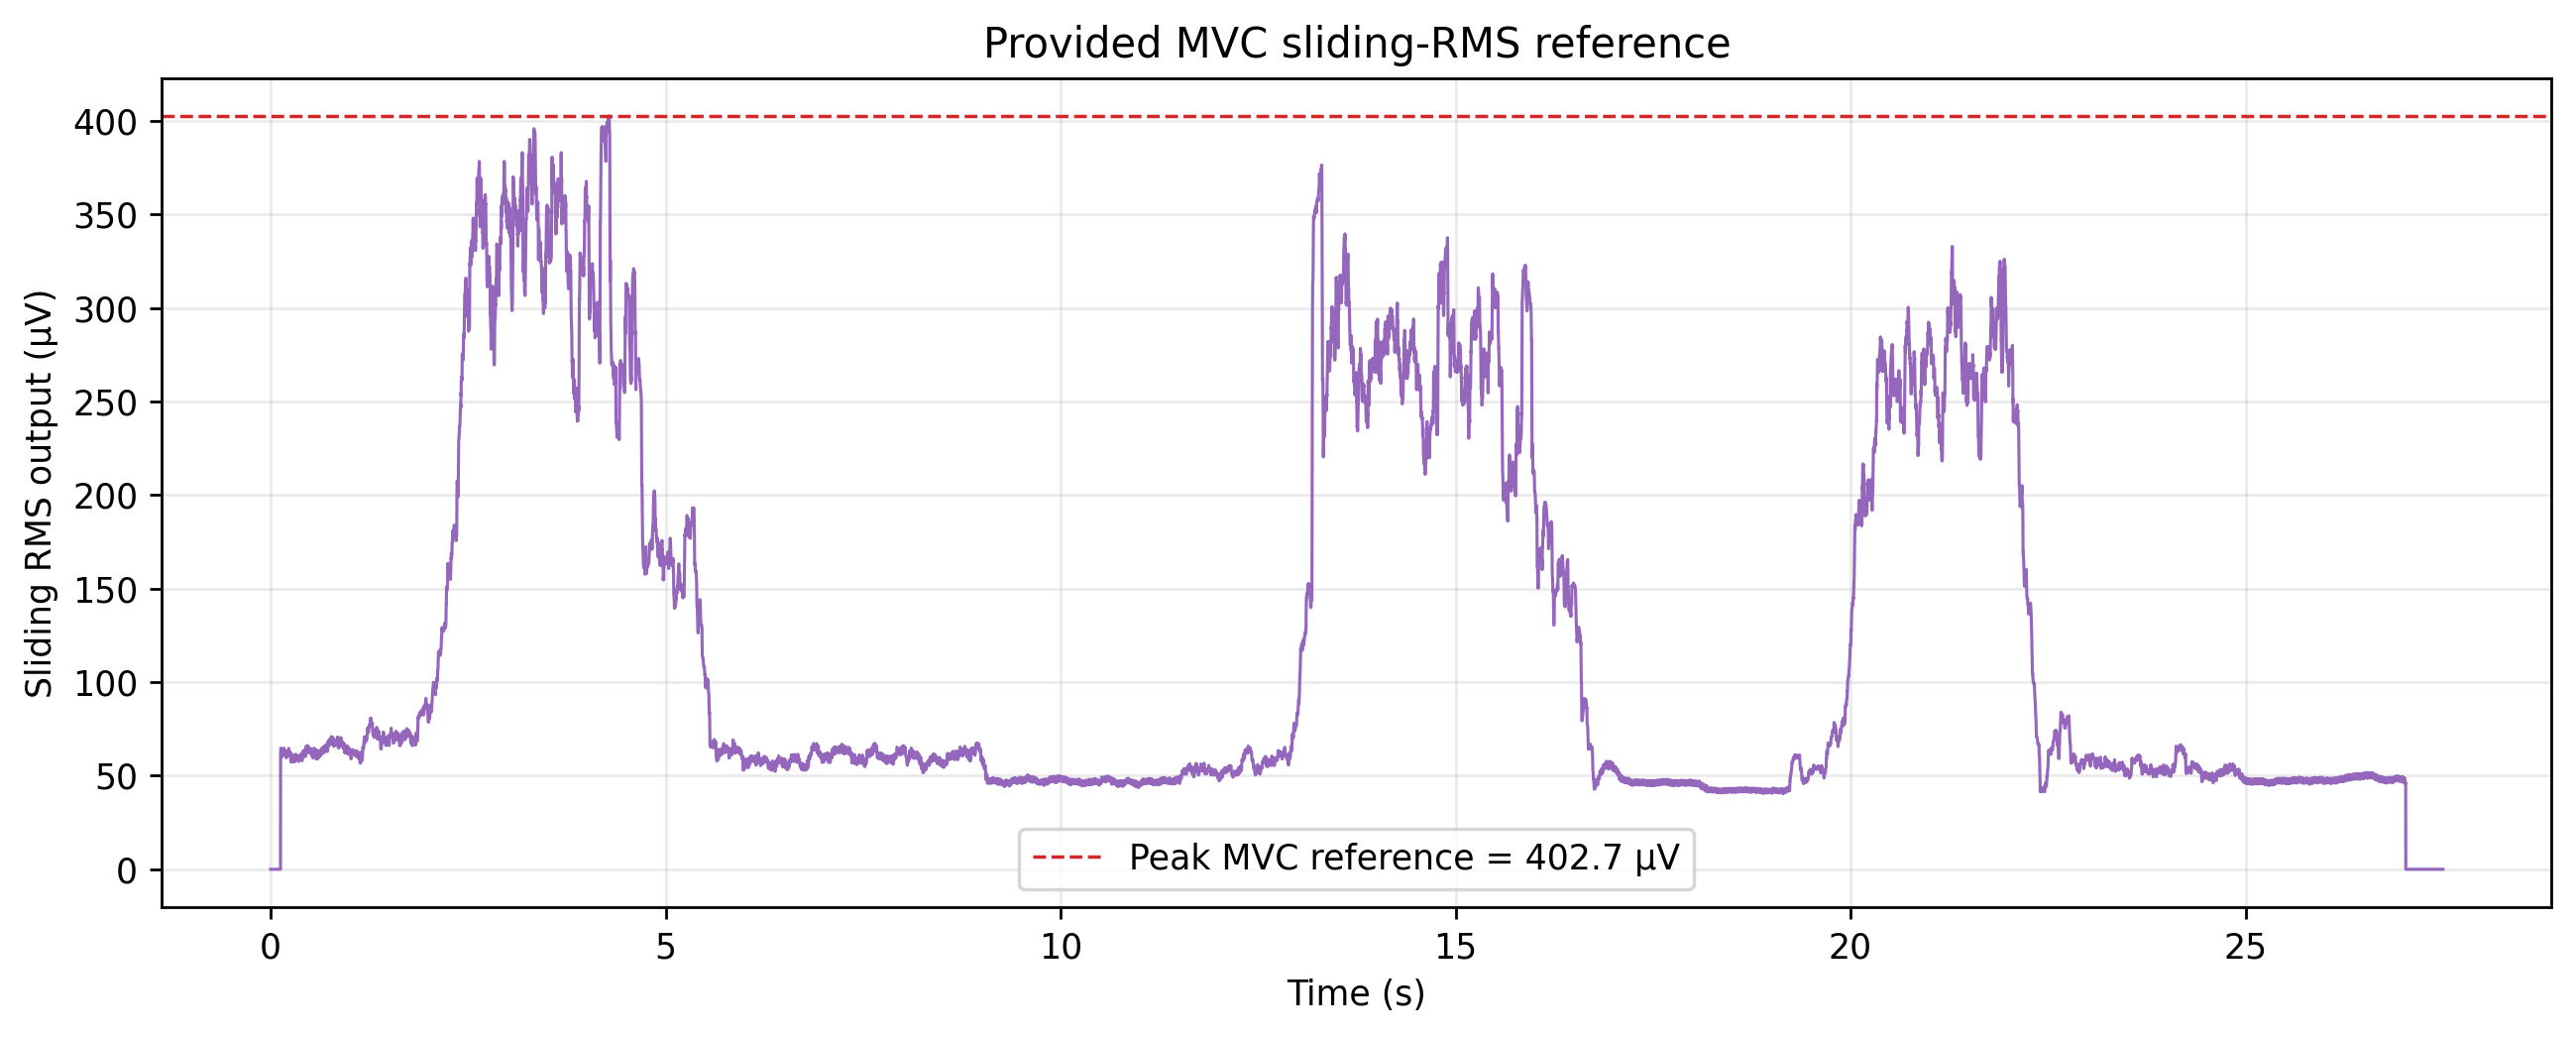
\includegraphics[width=0.96\textwidth]{emg_mvc_reference.png}
  \caption{Supplied MVC sliding-RMS reference signal and its peak value.}
  \label{fig:mvc-reference}
\end{figure}

\begin{figure}[H]
  \centering
  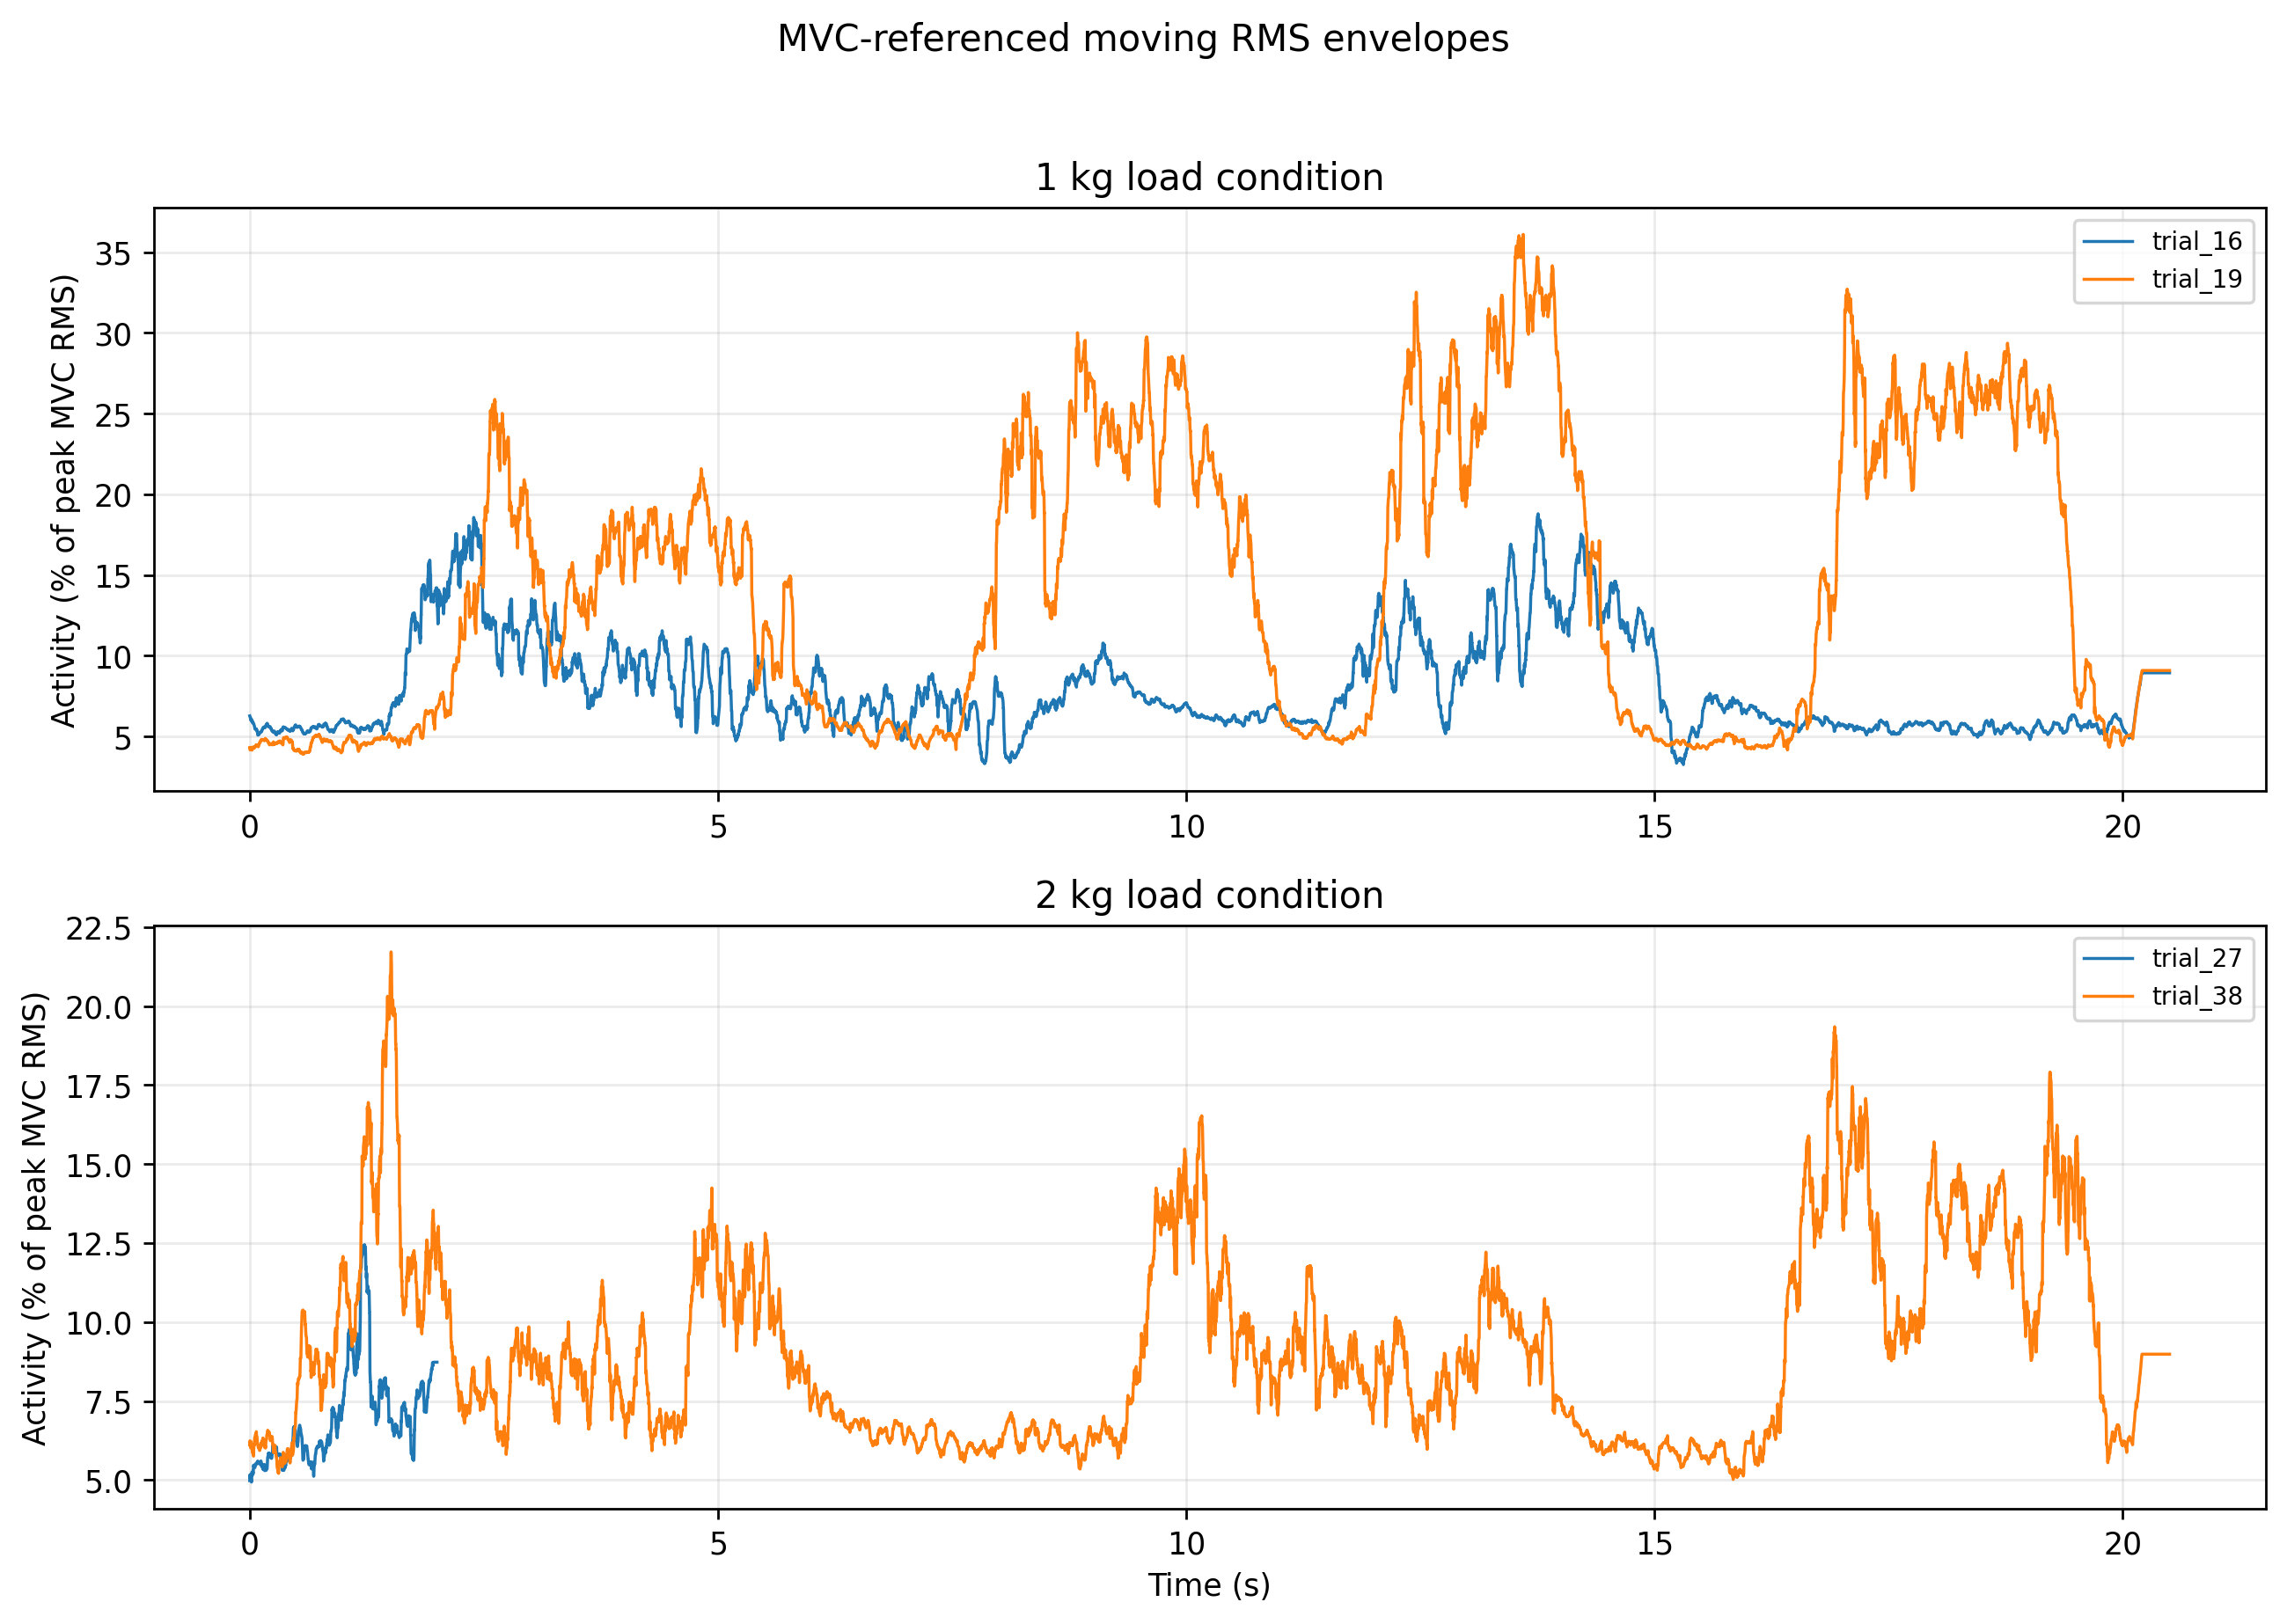
\includegraphics[width=0.96\textwidth]{emg_mvc_normalised_loads.png}
  \caption{Trial RMS envelopes expressed relative to the peak of the supplied MVC sliding-RMS reference.}
  \label{fig:mvc-normalised}
\end{figure}

\subsection{Per-recording summary}
Table~\ref{tab:trial-summary} lists the mean and peak moving-RMS values for each recording.
The comparison plot in Figure~\ref{fig:load-summary} shows the individual per-recording
mean RMS values and a horizontal marker for the mean of each load group.

\begin{table}[H]
\centering
\caption{Measured RMS features calculated from the supplied raw traces.}
\label{tab:trial-summary}
\small
\begin{tabularx}{\textwidth}{>{\raggedright\arraybackslash}p{0.27\textwidth} >{\centering\arraybackslash}p{0.10\textwidth} >{\centering\arraybackslash}p{0.15\textwidth} >{\centering\arraybackslash}p{0.15\textwidth} >{\centering\arraybackslash}X}
\toprule
\textbf{Recording} & \textbf{Load} & \textbf{Duration (s)} & \textbf{Mean RMS (\uV)} & \textbf{Peak RMS (\uV)} \\
\midrule
Trial 16 & 1 kg & 20.50 & 32.05 & 75.66 \\
Trial 19 & 1 kg & 20.50 & 58.49 & 145.33 \\
Trial 27 & 2 kg & 2.00 & 28.28 & 50.13 \\
Trial 38 & 2 kg & 20.50 & 36.74 & 87.43 \\
\bottomrule
\end{tabularx}
\end{table}

\begin{figure}[H]
  \centering
  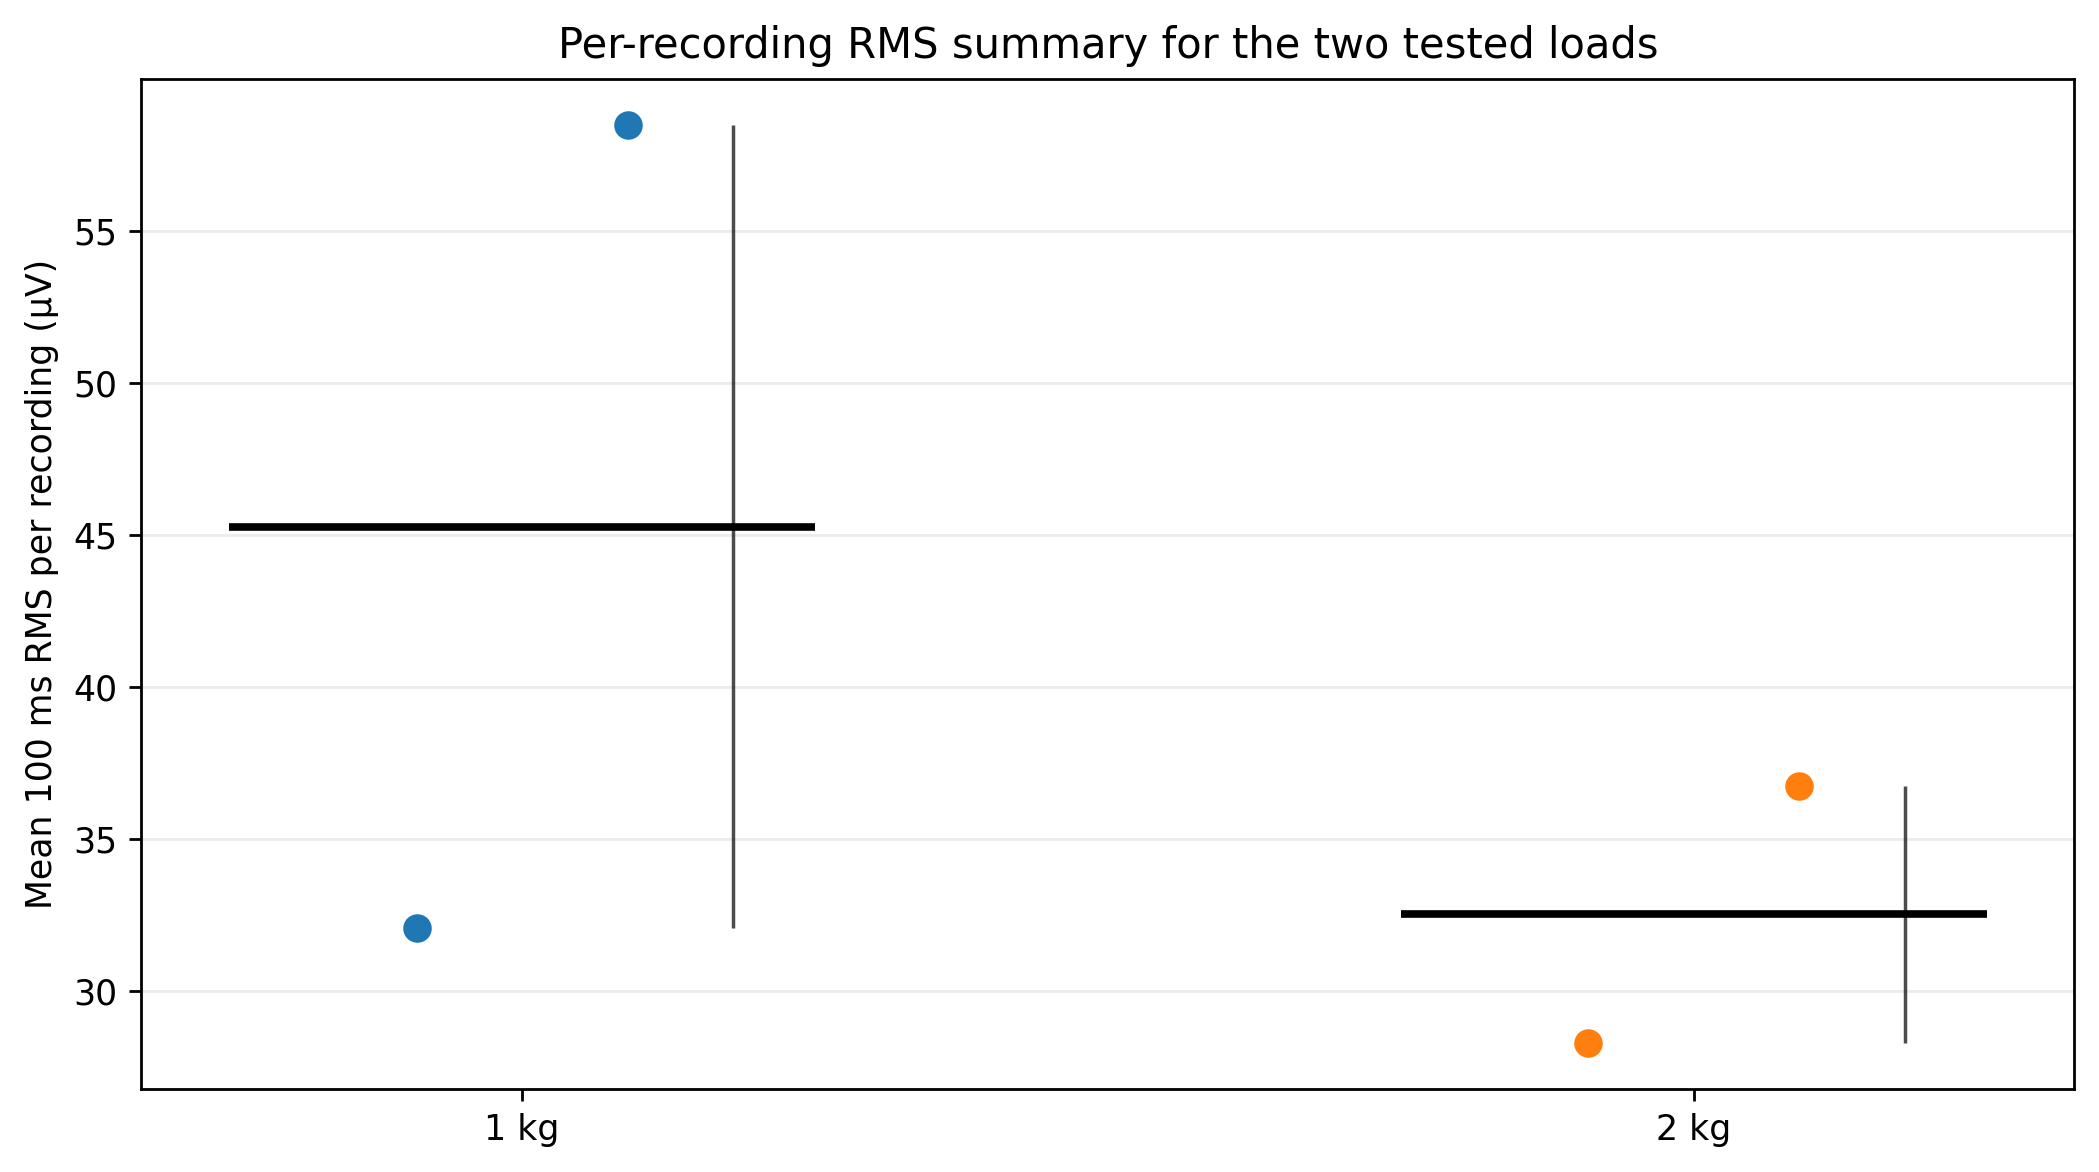
\includegraphics[width=0.88\textwidth]{emg_load_rms_summary.png}
  \caption{Mean 100 ms RMS for each recording, grouped by the two load conditions. Dots show individual recordings and black horizontal markers show the group means.}
  \label{fig:load-summary}
\end{figure}

\section{Discussion}
The results demonstrate why both raw EMG and an amplitude envelope are useful. The raw
signals preserve the recorded waveform and are helpful for identifying abrupt artefacts
or baseline shifts. The moving RMS envelopes summarise local signal amplitude, making
it easier to compare activation levels without following every oscillation in the raw
signal.

Under the current trial-to-load grouping, the mean of the per-recording mean RMS values
is approximately \(45.27\uV\) for the 1 kg condition and \(32.51\uV\) for the 2 kg condition.
These results do not show a simple increase in EMG amplitude with the larger external
load. This should not be interpreted as evidence that a 2 kg load necessarily requires
less muscle activation: only two recordings are assigned to each load, trial 27 lasts
only two seconds, and differences in movement execution, electrode contact, fatigue, or
recording quality may influence EMG amplitude. In addition, the load assignments must be
verified against the laboratory notes because the CSV metadata does not encode the loads.

The supplied MVC reference permits a relative-amplitude comparison, but the software's
exact sliding-RMS settings are not recorded in the file header. Consequently, the
MVC-referenced values are useful for visual comparison in this practical but are not a
fully validated standardised \%MVC outcome. A stronger comparison would use repeated
trials of equal duration, consistent movement speed and posture, confirmed load labels,
and the same explicitly documented preprocessing pipeline for both trial and MVC data.

\section{Conclusion}
This report examines surface EMG recordings from two external load conditions only: 1 kg
and 2 kg. Four raw files were grouped as two recordings per condition, and each raw signal
was converted to a 100 ms moving RMS envelope after removing its mean. The supplied MVC
sliding-RMS trace was used as a reference for relative amplitude plots. The trial results
show noticeable variation between recordings, so the group difference should be
interpreted cautiously, particularly because one 2 kg recording lasts only two seconds.
Before final submission, the trial-to-load mapping should be confirmed against the
laboratory record.

\end{document}
